\documentclass[a4j,dvipdfmx]{jsarticle}
\usepackage{graphicx}
%\usepackage{multirow}
%\usepackage{color}
%\usepackage{lscape}
%\usepackage{ascmac}
%\usepackage{txfonts}


\usepackage{listings, jlisting}
\renewcommand{\lstlistingname}{リスト}
\lstset{
  language={C},
  basicstyle=\ttfamily\scriptsize,
  commentstyle=\textit,
  classoffset=1,
  keywordstyle=\bfseries,
  frame=tRBl,
  framesep=5pt,
  showstringspaces=true,
  numbers=left,
  stepnumber=1,
  numberstyle=\tiny,
  tabsize=2
}


%% %subsubsubsectionの定義(できるだけ使わない方向で)
%% \makeatletter
%% \newcommand{\subsubsubsection}{\@startsection{paragraph}{4}{\z@}%
%%   {1.0\Cvs \@plus.5\Cdp \@minus.2\Cdp}%
%%   {.1\Cvs \@plus.3\Cdp}%
%%   {\reset@font\sffamily\normalsize}
%% }
\makeatother
\setcounter{secnumdepth}{4}
%ここまでsubsubsubsectionの定義

\begin{document}

\title{計算機科学実験及び演習4\\コンピュータグラフィックス\\課題1}
\author{工学部情報学科3回生 1029255242\\勝見久央}
\date{作成日: \today} % コンパイル時の日付が自動で挿入される
\maketitle
%文字コードはUTF-8推奨.それ以外ではline2のcontentsline~にエラー発生.
%選択範囲コメントアウトは選択中にM-;
%%%%%%%%%%%%%%%%%%%%%%%%%%%%%%%%%%%%%%%%%%%%%%%%%%%%%%%%%%%%%%%%%%%%%%
%ソースコードの貼付け
%% \lstinputlisting[caption=キャプション,label=ラベル,breaklines=true]
%% {./kadai01.sc}
%%次でも可
%% \begin{lstlisting}
%% \end{lstlisting}
\section{概要}
本実験課題では3Dポリゴンデータを透視投影によって投影したPPM画像を生成する
プログラムをC言語で作成した.

\section{要求仕様}
作成したプログラムが満たす仕様は以下の通りである.
\begin{itemize}
\item ポリゴンデータはプログラム内部で与え、頂点座標をランダムに生成する.
\item PPM画像の大きさは$256 \times 256$
\item カメラ位置は(x,y,z) = (0.0, 0.0, 0.0)
\item カメラ方向は(x,y,z) = (0.0, 0.0, 1.0)
\item カメラ焦点距離は256.0
\item ポリゴンには拡散反射を施す
\end{itemize}

\section{プログラムの仕様}
\subsection{留意点}
座標、RGB値等は、データ型をdoubleとして計算し、RGB値については、出力時に
一旦round関数を用いて丸めてint型に変換した後、char型に変換して出力した.
各点の座標については、double型のサイズ3の配列にxyz座標を格納して処理した.
プログラム内には頂点座標の例として2パターン分もコメントで記述している.
大文字アルファベットの定数はマクロである.


\subsection{各種定数}
%======================================================================
\subsubsection{ppm}
次の定数はppmファイル生成のための定数である.
\begin{itemize}
\item FILENAME\\
  ファイル名を指定. ここではimage.ppmaとしている.
  
\item MAGICNUM\\
  ppmファルのヘッダに記述する識別子. P3を使用.
  
\item WIDTH, HEIGHT, WIDTH\_STRING, HEIGHT\_STRING\\
  出力画像の幅、高さ. ともに256とする. STRINGは文字列として使用するためのマクロ.
  以降も同様.
  
\item MAX, MAX\_STRING\\
  RGBの最大値. 255を使用.

\end{itemize}

%======================================================================
\subsubsection{ポリゴンデータ}
次の定数はポリゴンデータとして定める定数である.
\begin{itemize}
\item VER\_NUM\\
  ポリゴンの頂点数
  
\item SUR\_NUM\\
  ポリゴンを生成する三角形平面の数
  
\item ver[VER\_NUM][3]\\
  VRMLのCoordinateノードのpointフィールドの値.
  ポリゴンを形成する各点の座標を格納する.
  点iの座標は(sur[i][0], sur[i][1], sur[i][2])
  である. 初期化はmain関数内で行う.
  double型2次元配列.
  
\item sur[SUR\_NUM][3]\\
  VRMLのIndexedFaceSetノード内のcoordIndexフィールドの値.
  ポリゴンを形成する三角形を指定する.
  三角形は点sur[i][0]、sur[i][1]、sru[i][2]の3点
  からなる.int型2次元配列.
  
\item diffuse\_color[3]\\
  VRMLのMaterialノードのdiffuseColorフィールドの値.
  配列の先頭から順にRGB値を表す.
  double型配列.
\end{itemize}


%======================================================================
\subsubsection{環境設定}
次の定数は光源モデルなどの外部環境を特定する定数である.
\begin{itemize}
\item FOCUS\\
  カメラの焦点距離. 256.0と指定.
  
\item light\_dir[3]\\
  光源方向ベクトル.doubel型配列.
  
\item light\_rgb[3]\\
  光源の明るさを正規化したRGB値にして配列に格納したもの.
  double型配列.
  
\end{itemize}

%======================================================================
\subsubsection{その他}
\begin{itemize}
\item image[HEIGHT][WIDTH]\\
  描画した画像の各点の画素値を格納するための領域.
  領域確保のみで初期化は関数内で行う.
  double型の3次元配列.
  
\item projected\_ver[VER\_NUM][2]\\
  画像平面上に投影された各点の座標を格納するための領域.
  領域確保のみで初期化は関数内で行う.
  また、最初にmain関数内で全ての点が黒になるように
  初期化を行ってから、シェーディングの結果をその上に反映させていく形をとる.
  double型2次元配列.
\end{itemize}

%======================================================================

\subsection{関数外部仕様}
\subsubsection{double func1(double *p, double *q, double y)}
double型2次元配列で表された2点p、qの座標とdouble型の値yを引数に取り、
直線pqと直線y=yの交点のx座標をdouble型で返す関数.
ラスタライズの計算を簡素化するために三角形を分割する際に主に用いる.

\subsubsection{int lineOrNot(double *a, double *b, double *c)}
double型2次元配列で表された3点a、b、cが一直線上にあるかどうかを判別する関数.
一直線上にある場合はint型1を返し、それ以外のときはint型0を返す.
後述の関数shadingの中で用いる.

\subsubsection{void perspective\_pro()}
大域変数で与えられた頂点座標ver[VER\_NUM][3]の各点に対して透視投影(pespective project)
を行い、その結果をグローバル領域に確保された領域projected\_ver[VER\_NUM][2]に書き込む.

\subsubsection{void shading(double *a, double *b, double *c, double *n)}
画像平面上に投影されたduble型2次元配列で与えられた3点a、b、cに対してシェーディングを行う関数.
さらに、シェーディング時に拡散反射をコンスタントシェーディングで適用するために必要になる、3点a、b、c
から成るポリゴンの面の法線ベクトルをdouble型3次元配列の形にしたnを引数にとる.
シェーディングの結果はグローバル領域にあるimage[HEIGHT][WIDTH]に書き込む.

\subsection{各関数のアルゴリズムの概要}
\subsubsection{double func1(double *p, double *q, double y)}
2点p、qを通る直線の方程式を求めて、直線y=yとの交点を計算する.
なお直線pqがx軸に平行の時はエラーが発生する.

\subsubsection{int lineOrNot(double *a, double *b, double *c)}
まず最初に3点a、b、cのx座標が全て同じであるかどうかを判定し、同じであれば一直線上にあると判定する.
同じでなければ、次に点cの座標を直線abの方程式に代入し、等号が成立するかどうかで一直線上に
あるかどうかを判定する。

\subsubsection{void perspective\_pro()}
実験資料の数式通りに全ての頂点に対して透視投影を適用する.
なお、このプログラムでは、撮像平面の中心が出力後の画像の原点に来るように、
投影後の点の座標のxy座標に$MAX/2$を加えて平行移動を施している.

\subsubsection{void shading(double *a, double *b, double *c, double *n)}
この関数内部では処理を単純化するため、処理の最初の段階で引数として与えられた3点が形成する
三角形の形と3点の位置関係を明らかにしておく必要がある.
なお、3点が一直線上にあればシェーディングの必要が無いため、この関数での処理は終了する.
\begin{figure}[b]
  \begin{center}
        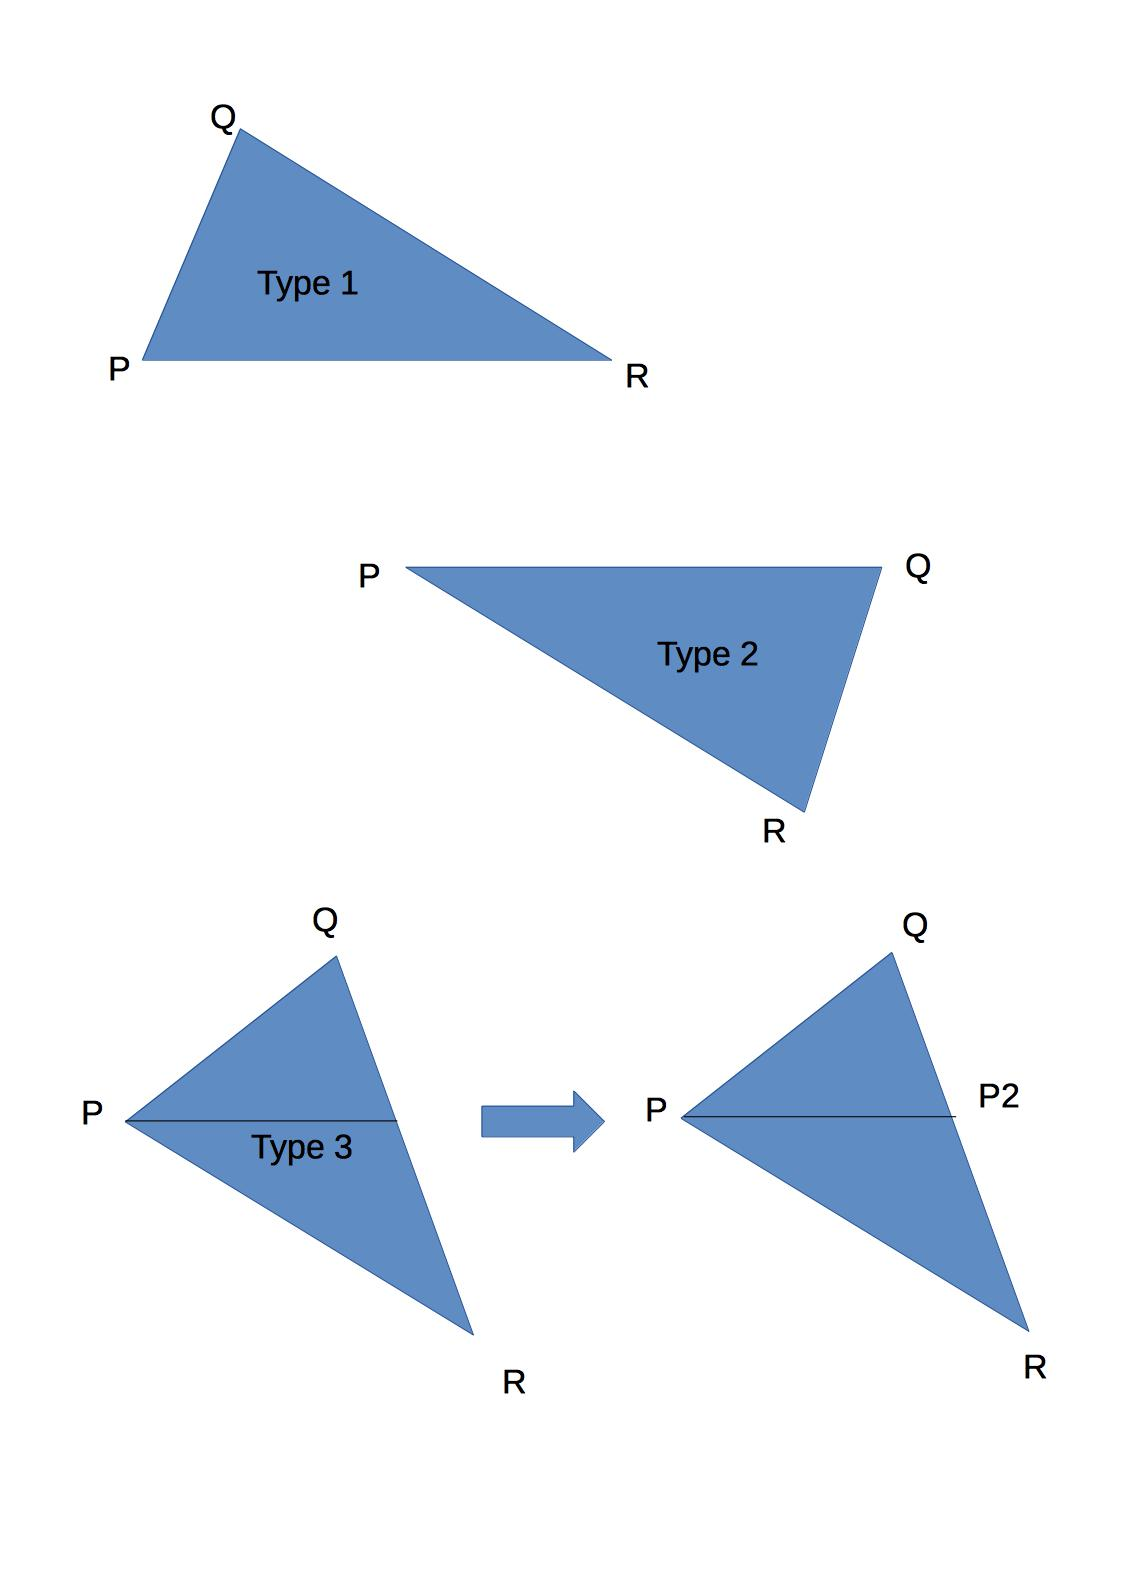
\includegraphics[clip,scale=0.3]{images/tritypes.eps}
        \caption{三角形の場合分け}
        \label{fig:tritypes}
  \end{center}
\end{figure}
このため、3点の位置関係に応じて以下の判別処理を行う.
\begin{itemize}
\item 与えられた3点a、b、cのy座標が小さい順にr、p、qと名前を変更する
\item 与えられた3点からなる三角形が分割して処理可能な三角形かどうかを判別する\\
  
  ⇒分割できないときは
  \begin{itemize}
  \item 「pとrのy座標が同じ」もしくは「pとqのy座標が同じ」のどちらかを判別する\\
  \item 前の手順で場合分けを行ったpとr、もしくはpとqの2点でx座標がpの方が
    小さくなるよう、必要に応じて名前を入れ替える.\\
    以上により三角形は図\ref{fig:tritypes}に示される、
    Type1とType2のどちらであるかが確定する.
  \end{itemize}
  
  ⇒分割できるときは
  \begin{itemize}
  \item 三角形を分割し、それぞれの三角形を形成する3点に適当な名前をつけて
    再びshading関数に引き渡す.\\
    これにより三角形は図\ref{fig:tritypes}に示されるようにType3に分類されるとわかる.
  \end{itemize}
\end{itemize}
以上の処理を行って、三角形の形がType1〜3のいずれに分類されるかを判別し、それぞれを別々に
処理する.また、シェーディングはコンスタントシェーディングで拡散反射を適用し、
各画素の輝度値を計算していく.


\section{プログラム本体}
プログラム本体は次のようになった.
\lstinputlisting[caption=キャプション,label=ラベル,breaklines=true]{./kadai01.c}


\section{実行例}
ランダム座標の描画を行った結果が図\ref{fig:random}、
\begin{figure}[htbp]
  \begin{center}
        
\includegraphics[clip,scale=0.7]{images/random.eps}
        \caption{ランダム座標の出力結果}
        \label{fig:random}
  \end{center}
\end{figure}
コメント内に記載されているav1.wrlの内容を出力した結果が図\ref{fig:av1}、
\begin{figure}[htbp]
  \begin{center}
        
\includegraphics[clip,scale=0.7]{images/av1.eps}
        \caption{av1.wrlの出力結果}
        \label{fig:av1}
  \end{center}
\end{figure}
av2の内容を出力した結果が図\ref{fig:av2}である.
\begin{figure}[htbp]
  \begin{center}
        
\includegraphics[clip,scale=0.7]{images/av2.eps}
        \caption{av2.wrlの出力結果}
        \label{fig:av2}
  \end{center}
\end{figure}



\section{問題点}
問題点としては、
初期段階でモジュール化をうまく考えなかったため、
グローバル変数を多用する事になってしまった点、
場合分けを多用しすぎてしまい、自分でもこれで必要十分なのかが把握できなくなってしまった点、
などが挙げられる.

\section{工夫点}
工夫した点としては、
コメントを随所に入れて見やすいコードを心がけた点、
マクロを多用して後でプログラムに変更を加えやすいようにした点、
ポリゴンデータなどの入力データは、勝手に書き換わらないようconstで宣言した点、
後々の課題で使えそうな処理をモジュール化して書いた点、
などが挙げられる.


\end{document}
